\section{Theorie}

    \subsection{Zielsetzung}

        \noindent In diesem Versuch werden unterschiedliche abgeglichene Brückenschaltungen als Messaperaturen betrachtet. Es lässt sich 
        jede physikalische Größe die sich als elektrischen Widerstand darstellt werden kann, messen. 

    \subsection{Allgemeine Brückenschaltung}

        \begin{figure}[ht]
            \centering
            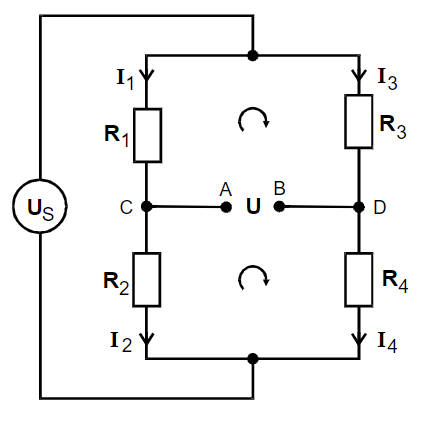
\includegraphics[width=0.5\textwidth]{latex/images/Prinzip_Brueck.PNG}
            \caption{Prinzipielle Brückenschaltung\protect \cite{V302}.}
            \label{img:Prinzip}
        \end{figure}

        \noindent In Abbildung(\ref{img:Prinzip}) ist eine allgemeine Brückenschaltung zu sehen, mittels der Potentialdifferenz kann nun ein 
        Verhältnis der Widerstände bestimmt werden. Dies geschiet mittels dem ersten Kirchhoffschen Gesetz, der Knotenregel welches besagt, 
        dass der Strom der in einen Knoten fließt gleich dem Strom ist, der aus dem Knoten raus fließt. Es ist also 

        \begin{equation*}
            I_1 = I_2 \quad \quad \text{und} \quad \quad I_3 = I_4 ,
        \end{equation*}

        \noindent aus dem zweiten Kirchhoffschen Gesetz, der Maschenregel welche besagt, dass die Summe aller Spannungen innerhalb einer Masche 
        gleich 0 ist, folgt 

        \begin{align*}
             U &= -R_1 I_1 + R_3 I_3 \\
            -U &= -R_2 I_2 + R_4 I_4 .
        \end{align*}

        \noindent Einsetzten von der Speisespannung $U_{\text{S}} = I_1 (R_1 + R_2)$ und umstellen ergibt 

        \begin{equation*}
            U = \frac{R_2 R_3 -R_1 R_4}{(R_3 + R_4)(R_1 + R_2)} U_{\text{S}}.
        \end{equation*}

        \noindent Gilt also 
        
        \begin{equation}
         R_2 R_3 = R_1 R_4,
        \label{eq:Widerstand}
        \end{equation}
        \noindent verschwindet die Brückenspannung unabhängig von der Speisespannung, die Brücke ist 
        abgeglichen.


   % \subsection{Brückenschaltungen mit komplexen Widerständen}

        

    \subsection{Spezielle BrückenschaItungen}

        \noindent Brückenschaltungen können weiterhin auch zur Vermessung elektrischer Bauteile genutzt werden, einige davon 
        sind im folgenden aufgelistet.

        \subsubsection{Wheatstonesche Brücke (Widerstandsmessbrücke)}

            \begin{figure}[ht]
                \centering
                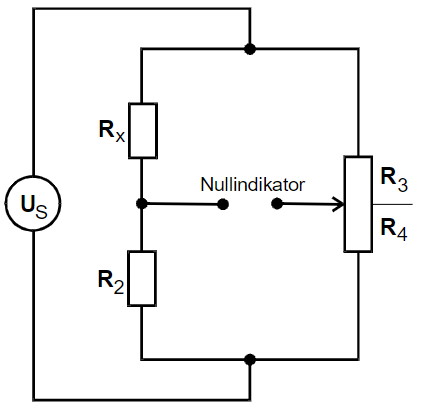
\includegraphics[width=0.5\textwidth]{latex/images/Wheat.PNG}
                \caption{Wheatstonesche Brückenschaltung\protect \cite{V302}.}
                \label{img:Wheat}
            \end{figure}

            \noindent Die Wheatstonsche Brückenschaltung aus Abbildung(\ref{img:Wheat}) besteht genau wie die bereits angeschaute allgemeine 
            Brückenschaltung(\ref{img:Prinzip}) nur aus ohmschen Widerständen und wird benutzt um den Widerstand $R_x$ zu bestimmen. 
            Nach Formel(\ref{eq:Widerstand}) ergibt sich schnell 

            \begin{equation}
                R_x = R_2 \frac{R_3}{R_4}
            \end{equation}

            \noindent für den unbekannten Widerstand.

        \subsubsection{Kapazitätsmessbrücke}

            \noindent Kondensatoren besitzten in der Realität neben ihrer Kapazität auch immer einen Widerstand, da sie elektrische Energie 
            in Wärme transformieren, daher werden ideale Kondensatoren in Ersatzschaltbildern noch mit einem fiktiven Widerstand versehen. 
            Um nun den Widerstand und die Kapazität dieses realen Kondensators zu bestimmen, eignet sich die Schaltung aus 
            Abbildung(\ref{img:Kapa}).

            \begin{figure}[ht]
                \centering
                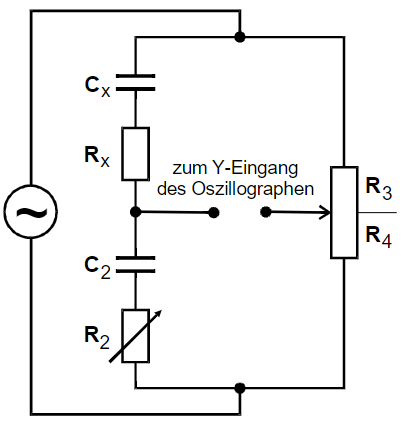
\includegraphics[width=0.5\textwidth]{latex/images/Kondensator.PNG}
                \caption{Eine Kapazitätsmessbrücke\protect \cite{V302}.}
                \label{img:Kapa}
            \end{figure}

            \noindent Hier ist $R_2$ ein veränderlicher Widerstand um die Phasenverschiebung des fiktiven Widerstandes auszugleichen. 
            Es ergibt sich 

            \begin{equation*}
                R_x = R_2 \frac{R_3}{R_4}
            \end{equation*}

            \noindent und 

            \begin{equation*}
                C_x = C_2 \frac{R_4}{R_3}
            \end{equation*}

            \noindent für die Eigenschaften des realen Kondensators.

        \subsubsection{Induktivitätsmessbrücke}

            \noindent Analog zu den Kondensatoren, haben auch reale Spulen neben der Induktivität einen Widerstand der im Ersatzschaltbild durch 
            einen fiktiven Widerstand dargestellt wird. 

            \begin{figure}[ht]
                \centering
                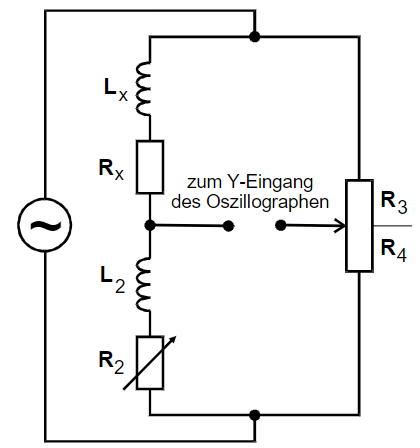
\includegraphics[width=0.5\textwidth]{latex/images/Spule.PNG}
                \caption{Eine Induktivitätsmessbrücke\protect \cite{V302}.}
                \label{img:Spul}
            \end{figure}

            \noindent Zur Bestimmung der Induktivität $L_x$ und des Widerstandes $R_x$ einer realen Spule kann eine Schaltung wie in 
            Abbildung(\ref{img:Spul}) verwendet werden. Die Formeln für den Widerstand ergeben sich Analog zu denen der Kapazitätsmessbrücke zu 

            \begin{equation*}
                R_x = R_2 \frac{R_3}{R_4},
            \end{equation*}

            \noindent für den fiktiven Widerstand und 

            \begin{equation*}
                L_x = L_2 \frac{R_3}{R_4}
            \end{equation*}

            \noindent für die Induktivität. In dieser Schaltung bekommt nur die zu vermessende Spule einen fiktiven Widerstand, die Spule 
            $L_2$ wird jedoch als ideale Spule genähert, dies ist gerade für kleine Spulen nicht realisierbar. Dieses Problem wird mit der 
            Maxwell-Brücke überwunden.

        \subsubsection{Induktivitätsmessung mittels Maxwell-Brücke}

            \noindent Das Schaltbild der bereits erwähnten Maxwell-Brücke ist in Abbildung(\ref{img:Max}) zu finden.

            \begin{figure}[ht]
                \centering
                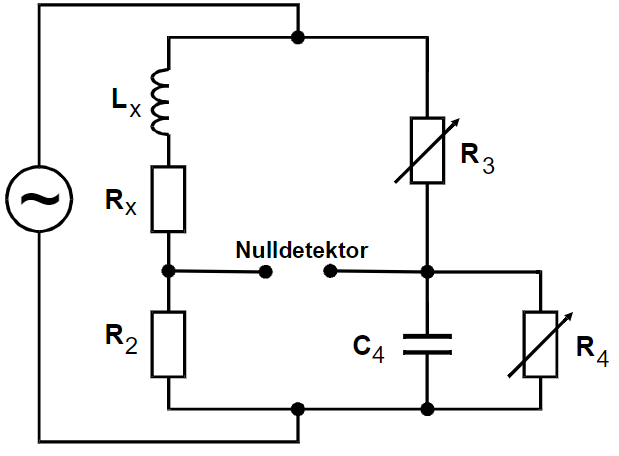
\includegraphics[width=0.5\textwidth]{latex/images/Maxwell.PNG}
                \caption{Eine Maxwell-Brücke \protect \cite{V302}.}
                \label{img:Max}
            \end{figure}

            \noindent Hier sind $R_3$, $R_4$ regelbare Widerstände und $C_4$ ein möglichst verlustarmer Kondensator.
            Hier raus ergibt sich 

            \begin{equation*}
                R_x = \frac{ R_2 R_3}{R_4}
            \end{equation*}

            \noindent und

            \begin{equation*}
                L_x = R_2 R_3 C_4.
            \end{equation*}

            \noindent In diesen Formeln entsteht keine Frequenzabhängigkeit, jedoch besitzt die Maxwell-Brücke einen optimalen Frequenzbereich 
            da die realen Bauteile eine Streukapazität aufweisen. 

        \subsubsection{Wien-Robinson-Brücke}

            \noindent In Abbildung(\ref{img:Wien}) ist das Schaltbild einer Wien-Robinson-Brücke aufgezeichnet. Hier werden keine 
            Abgleichelemente benötigt da in dieser Schaltung durch die Frequenz abgeglichen wird. Somit werden nun die zum Teil 
            komplexen Impedanzen der vier Zweige 

            \begin{align*}
                Z_1 &= 2R' \\
                Z_2 &= R'\\
                Z_3 &= R + \frac{1}{ i \omega C}\\
                Z_4 &= \frac{R}{1 + i \omega R C}
            \end{align*}

            \noindent benötigt. Mittels der Maschenregel ergibt sich dann für das Verhältnis aus Brückenspannung $U_{\text{Br}}$ 
            und Speisespannung $U_{\text{Sp}}$ 

            \begin{equation*}
                \left|  \frac{U_{\text{Br}}}{U_{\text{Sp}}} \right|^2 = \frac{1}{9} 
                \cdot \frac{\left(\omega^2 R^2 C^2 - 1\right)^2}{\left(1 - \omega^2 R^2 C^2\right)^2 + 9 \omega^2 R^2 C^2} .
            \end{equation*}

            \begin{figure}[ht]
                \centering
                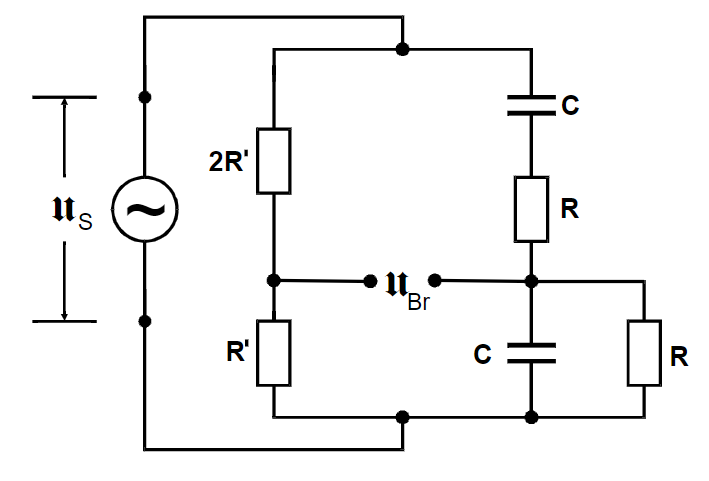
\includegraphics[width=0.5\textwidth]{latex/images/Wien.PNG}
                \caption{Schaltbild einer Wien-Robinson-Brücke \protect \cite{V302}.}
                \label{img:Wien}
            \end{figure}

            \noindent Dieses Verhältnis nähert sich für $\omega_0 = \frac{1}{RC}$ Null an. Weiterhin entsteht mittels der 
            Substitution $\Omega = \frac{\omega}{\omega_0}$ die Gleichung

            \begin{equation}
                \left| \frac{U_{\text{Br}}}{U_{\text{Sp}}} \right|^2 = \frac{1}{9} \cdot 
                \frac{\left(\Omega^2 - 1\right)^2}{\left(1 - \Omega^2\right)^2 + 9 \Omega^2}.
            \end{equation}

            \noindent Nun ist schnell zu erkennen, dass die Wien-Robinson-Brücke Frequenzen um $\omega_0$ raus filtert.







